\documentclass[10pt]{BHCexam}
%\usepackage{morelull}
\usepackage{tkz-euclide}
\usepackage{subfigure} 
\biaoti{霍邱县~$2019 \sim 2020$学年度第一学期期中考试}
\fubiaoti{\zihao{-2}七年级数学试卷}
\begin{document}
\maketitle
\mininotice
\begin{questions}
%选择题
%{\heiti 一、选择题}{\kaishu (本大题共有$10$小题,每小题$4$分,共计$40$分)}
\xuanze
\qs $2019$的相反数是\xx
\onech{$2019$}{$-2019$}{$\dfrac{1}{2019}$}{$-\dfrac{1}{2019}$}
\qs 下列为同类项的一组是\xx
\onech{$7$与$-\dfrac{1}{3}$}{$-xy^2$与$\dfrac{1}{4}yx^2$}{$x^3$与$2^3$}{$ab$与$7a$}
\qs 餐桌边的一蔬一饭,舌尖上的一饮一酌,实属来之不易,舌尖上的浪费让人触目惊心.据统计,中国每年浪费的食物总量折合粮食约为$500$亿千克,这个数据用科学计数法表示为\xx
\onech{$5\times 10^9$千克}{$5\times 10^{10}$千克}{$50\times 10^9$千克}{$0.5\times 10^{11}$千克}
\qs 下列方程中是一元一次方程的是\xx
\twoch{$3x-2=4x+\dfrac{1}{2}$}{$x^2-3x=1$}{$3-\dfrac{1}{x}=4$}{$6-3x=4+y$}
\qs 用四舍五入法按要求对$0.05049$分别取近似值,其中错误的是\xx
\twoch{$0.1(\kaishu\text{精确到}0.1)$}{$0.05(\kaishu\text{精确到百分位})$}{$0.051(\kaishu\text{精确到千分位})$}{$0.050(\kaishu\text{精确到}0.001)$}
\qs 下列去括号运算正确的是\xx
\twoch{$-(2x+5)=-2x+5$}{$-\dfrac{1}{2}(4x-2)=-2x+2$}{$\dfrac{1}{3}(2m-3n)=\dfrac{2}{3}m+n$}{$-(\dfrac{2}{3}m-2x)=-\dfrac{2}{3}m+2x$}
\qs 已知$n$为整数,$x^{2+n}-y^2+1$是二次三项式,则$n$应当取的值是\xx
\onech{$-1$}{$0$}{$1$}{$0\text{或}-1$}

\begin{minipage}[t]{0.7\textwidth}%并排放两张图片,每张占页面的0.5,下同。
\vspace*{-2cm}  
\qs 有$12$米长的木料,要做成一个如图所示的窗框({\kaishu 一个大长方形中间有一横档}),如果假设窗框横档的长度为$x$米,那么窗框的面积是多少平方米?({\kaishu 不考虑窗框和横档的厚度})\xx
\onech{$x(6-x)$}{$x(12-x)$}{$x(6-3x)$}{$x(6-\dfrac{3}{2}x)$}
\end{minipage}  
\begin{minipage}[t]{0.3\textwidth}  
		\centering
		%\includegraphics{qinianji-2}
		\begin{tikzpicture}
		\tkzDefPoints{0/0/A,3/0/B,0/-2/D,3/-2/C}
		\tkzDefPoints{0/-0.7/E,3/-0.7/F}
		\tkzDrawPolygon[very thick](A,B,C,D)
		\tkzDrawSegment[very thick](E,F)
		\tkzDrawSegment[dim={$x$米,-10pt,}](E,F)
	
\end{tikzpicture}
\end{minipage}	
%\vspace*{-1.3cm}
\qs 数$a,b$在数轴上的位置如图所示,则下列结论中:\ding{192}$ab<0$;\ding{193}$a+b<0$;\ding{194}$a-b<0$;\ding{195}$a<\abs{b}$;\ding{196}$-a>-b$.其中正确的有\xx
\onech{$2$个}{$3$个}{$4$个}{$5$个}
	
\begin{center}
	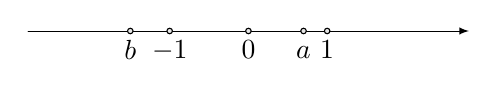
\begin{tikzpicture}
	\tkzDefPoints{-2/0/A,-1.5/0/B,-1/0/D,0.7/0/C,1/0/E,2/0/F,0/0/O}
	\tkzDrawLine[->,>=latex](A,F)
	\tkzDrawPoints(B,D,C,E,O)
	\tkzLabelPoint[below](B){$b$}
	\tkzLabelPoint[below](D){$-1$}
	\tkzLabelPoint[below](O){$0$}
	\tkzLabelPoint[below=2pt](C){$a$}
	\tkzLabelPoint[below](E){$1$}
	\end{tikzpicture}
\end{center}

\qs 观察下列关于~$x$~的单项式,探究其中规律:~$x,3x^2,5x^3,7x^4,9x^5,11x^6,\cdots$~按照这个规律,第~$2019$~个单项式是\xx
\onech{$2019x^{2019}$}{$4037x^{2018}$}{$4037x^{2019}$}{$4039x^{2019}$}
\vspace{-2EM}
%填空题
\tiankong
\qs 一艘潜水艇所在的海拔高度为$-50m$,若一条鲨鱼在潜水艇下方$10m$处,则鲨鱼所在的海拔高度为\underline{~\hspace{2cm}~}.
\qs 如果关于$x$的方程$3x+4=0$与方程$3x+4k=18$是同解方程,则$k=$ \underline{~\hspace{2cm}~}.
\qs 规定$a\otimes b=ab-5a+2b$,则$(-4)\otimes 6$的值为\underline{~\hspace{2cm}~}.
\qs 判断下列变形,\ding{192}由$3x-1=2x+1$得$3x-2x=1+1$;\ding{193}由$2(x+1)=2y+1$得$x+1=y+1$;\ding{194}由$2a+3b=c-6$得$2a=c-9b$;\ding{195}由$a^2=b^2$得$a=b$或$a=-b$.其中正确的有:\underline{~\hspace{2cm}~}.
%解答题
\jianda
\qs {\kaishu(本题满分$8$分)}画出数轴,并在数轴上表示下列各数,最后用“$<$”将各数连接起来.
\begin{parts}
$-4$,$\abs{-2.5}$,$-(-2)$,$0$,$-1^2$
\end{parts}
\vspace{3cm}

\qs {\kaishu(本题满分$8$分)}计算:
\begin{parts}
$(1)-20+(-14)-(-18)$ \hspace{2cm}  $(2)\abs{5-8}+24\div (-2)^2\times \dfrac{1}{3}$
\end{parts}
\vspace{3cm}

\qs {\kaishu(本题满分$8$分)}解方程:
\begin{parts}
$(1)-2x+1=4x-1$ \hspace{3cm}  $(2)\dfrac{3x+2}{4}=\dfrac{2x-1}{3}$
\end{parts}
\vspace{3cm}

\qs {\kaishu(本题满分$8$分)}先化简,再求值:
\begin{parts}
$5(a^2b-ab^2-1)-(ab^2+3a^2b-5)$,其中$a=-\dfrac{1}{2},b=\dfrac{1}{3}$
\end{parts}

\vspace{3cm}
\qs {\kaishu(本题满分$10$分)}小明在进行期中复习归纳时发现近阶段学习了两个非负数$a^2$和$\abs{a}$($a$是任意有理数).于是他结合所学习的两个非负数的知识,自己编了一道题来考他的同桌:已知$\left(x+\dfrac{1}{3}\right)^2+\abs{y-2}=0$,求$x^y$的值,如果你是他的同桌,你能解答这个问题吗?

\vspace{5cm}

\qs {\kaishu(本题满分$10$分)}为节约用水,某地推行阶梯式水价计费制,标准如下:若每户每月用水不超过$15$立方米,则按每立方米$1.5$元计费;若超过$15$立方米,则超过部分按每立方米$2.5$元计费.
\begin{parts}
\part 小华家上月用水$m$立方米,请用含$m$的代数式表示:\\
\ding{192}若$m\leqslant 15$,则小华家应缴纳水费\underline{~\hspace{2cm}~}元;\\
\ding{193}若$m>15$,则小华家应缴纳水费\underline{~\hspace{2cm}~}元.
\part 小红家上月缴纳水费$40$元,试求小红家上个月用水多少立方米?
\end{parts}

\vspace{5cm}

\qs {\kaishu(本题满分$12$分)}老师在讲解算式$\abs{5-2}=3$时告诉我们:这个算式表示$5$与$2$两数之差的绝对值是$3$,实际上也可以理解为$5$与$2$两数在数轴上所对应的两点之间的距离是$3$个单位长度.请你结合以上知识解答以下问题:
\begin{parts}
\part 列式计算$-6$与$\dfrac{1}{2}$两数在数轴上所对应的两点之间的距离;
\part $x$与$-4$两数在数轴上所对应的两点之间的距离可以表示为\underline{~\hspace{2cm}~};
\part 找出所有符合条件的整数$x$,使得$\abs{x+4}+\abs{x-1}=5$,这样的整数是\underline{~\hspace{2cm}~}.
\end{parts}

\vspace{5cm}

\qs {\kaishu(本题满分$12$分)}在抗洪救灾中,部队官兵用冲锋舟沿东西方向的河流抢救灾民,早晨从$A$地出发,晚上到达$B$地,约定向东为正方向,当天航行路程记录如下:$12,-8,-16,-7,13,-6,10,-3$(单位:千米)
\begin{parts}
\part $B$地在$A$地何位置?
\part 若冲锋舟每千米耗油$0.05$升,求这次行动共耗油多少升?
\end{parts}

\vspace{7cm}
\qs {\kaishu(本题满分$14$分)}由绝对值的定义可知:一个正数的绝对值是它的本身;一个负数的绝对值是它的相反数;$0$的绝对值是$0$.现有一组数$x_1,x_2,x_3,\cdots,x_{2019}$都是不等于$0$的有理数,请你探究以下问题:
\begin{parts}
\part 若$y_1=\dfrac{\abs{x_1}}{x_1}$,求$y_1$的值;
\part 若$y_2=\dfrac{\abs{x_1}}{x_1}+\dfrac{\abs{x_2}}{x_2}$,求$y_2$的值;
\part 若$y_3=\dfrac{\abs{x_1}}{x_1}+\dfrac{\abs{x_2}}{x_2}+\dfrac{\abs{x_3}}{x_3}$,则$y_3=$\underline{~\hspace{2cm}~}({\kaishu 不需解答过程,直接写出结果});
\part 由以上探究可知,若$y_{2019}=\dfrac{\abs{x_1}}{x_1}+\dfrac{\abs{x_2}}{x_2}+\dfrac{\abs{x_3}}{x_3}+\cdots +\dfrac{\abs{x_{2019}}}{x_{2019}}$,则$y_{2019}$共有\underline{~\hspace{2cm}~}个不同数值.在$y_{2019}$这些不同数值中,最大的值与最小的值之间的差等于\underline{~\hspace{2cm}~}.
\end{parts}


\end{questions}
\end{document}